\documentclass{beamer}
\setbeamertemplate{section in toc}[sections numbered]
\usepackage[T1]{fontenc}
\usepackage[utf8]{inputenc}
\usepackage[italian]{babel}
\usepackage{amsmath}
\usepackage{amsfonts}
\usepackage{amssymb}
\usepackage{mathtools}
\usepackage{resizegather} \addtolength{\jot}{4pt}
\usepackage{caption} \captionsetup{tableposition=top,figureposition=bottom,font=small}
\usetheme{metropolis} \setbeamertemplate{bibliography item}[text]
%\usefonttheme{professionalfonts}

\DeclareMathOperator{\Realpart}{Re}
\renewcommand{\Re}{\Realpart}

\newcommand{\dx}{\, dx}
\newcommand{\dt}{\, dt}
\newcommand{\lj}{\lambda_j}
\newcommand{\norm}[1]{\left\lVert#1\right\rVert}
\newcommand{\norminf}[1]{\left\lVert#1\right\rVert_\infty}
\newcommand{\normtwo}[1]{\left\lVert#1\right\rVert_2}
\newcommand{\normltwo}[1]{\left\lVert#1\right\rVert_{L^2}}
\newcommand{\normhone}[1]{\left\lVert#1\right\rVert_{H^1}}
\newcommand{\R}{\mathbb{R}}
\newcommand{\seminorm}[1]{\left\lvert#1\right\rvert}

\title{Domain decomposition methods: a tool for the parallelization
	of large-scale simulations}
\subtitle{An introduction, with a focus on scalable methods for Poisson's equation
	(two-level overlapping AS).}
\author{Bruno Degli Esposti}
\date{January 2020 - Topics on control and numerics of PDEs}

\begin{document}

\begin{frame}
\maketitle
\end{frame}

\begin{frame}
\frametitle{Table of contents}
\tableofcontents
\end{frame}

\section{The importance of being scalable}
\begin{frame}
\frametitle{Linear, time indipendent PDE simulation pipeline}
\begin{itemize}%[<+->]
\item Mesh generation or loading
\item Linear system assembly ($Au=f$)
\item Essential boundary conditions
\item Preconditioner (optional)
\item Iterative sparse linear system solver
\item Postprocessing and visualization
\end{itemize}
\end{frame}

\begin{frame}
\frametitle{Scalability in the context of HPC}
Assumption: the linear system is too large to solve (or even assemble)
on a single CPU. We need a way to distribute work among multiple processors.
Moreover, we are looking for algorithms that satisfy a scalability property.
Let:
\begin{itemize}%[<+->]
\item $T$ be the total running time
%\item $n_\text{flop}$ be the total number of floating-point operations
\item $n$ be the size of the linear system $Au = f$
\item $n_\text{cores}$ be the number of parallel processors available
\end{itemize}
An algorithm is said to be (weakly) \emph{scalable} if
\[
\frac{n}{n_\text{cores}} \;\; \text{constant}
\implies T \;\; \text{constant}
\]
\end{frame}

\begin{frame}
\frametitle{Scalability in the context of HPC}
\begin{center}
Bad news: parallel programming is hard... \\[12pt]
\pause
...because we are used to thinking in terms of sequential tasks. \\[12pt]
\pause
An example? The pipeline itself! \\[12pt]
\pause
Also, iterative methods for the solution of the linear system.
\end{center}
\end{frame}

\begin{frame}
\frametitle{Scalability in the context of HPC}
Without preconditioners, iterative methods cannot scale:
as the size of the problem increases,
\begin{itemize}%[<+->]
\item The number of unknowns $n$ in the linear system increases
\item Hence, the condition number $k$ of $A$ increases
\item In turn, the number of iterations $n_\text{iter}$
	required to get a small residual increases
\item Since each iteration has a fixed cost, $T$ increases even if
	$n/n_\text{cores}$ remains constant.
\end{itemize}
The fix is a \emph{scalable} preconditioner, i.e.\ one that can
keep $n_\text{iter}$ bounded as the size of the problem grows.
\end{frame}

\section{What is domain decomposition?}
\begin{frame}
\frametitle{High-level overview of DDMs}
All kinds of domain decomposition methods work roughly like this:
\begin{itemize}%[<+->]
\item Split the domain $\Omega$ into $N$ %overlapping
	subdomains $\Omega_i$ ($N \approx n_\text{cores}$)
\item Assemble local matrices $A_i$ for each subdomain
\item Factorize each matrix $A_i$ using a direct method (e.g. LU)
\item Paste together the $A_i$ blocks to form a preconditioner $M$
\item Add a coarse space correction to $M$ for scalability (optional)
\end{itemize}
Now $M^{-1}y$ can be quickly computed using the factorizations.
\end{frame}

\begin{frame}
\frametitle{Linear, time indipendent PDEs simulation pipeline + DDM}
\begin{itemize}%[<+->]
\item Mesh generation or loading
\item \textbf{Mesh partitioning} (possibly automatic, with e.g.\ METIS)
\item Linear system assembly ($Au=f$)
\item Essential boundary conditions
\item Preconditioner $M$ \textbf{based on domain decomposition}
\item Iterative sparse linear system solver
\item Postprocessing and visualization
\end{itemize}
\end{frame}

\begin{frame}
\frametitle{Domain decomposition is:}
\begin{itemize}%[<+->]
\item A technique to calculate a scalable preconditioner in parallel
\item Compatible with most discretization schemes (FE,FD,FV,...)
\item Well-suited for heterogeneous or multiphysics problems
\item A way to improve the robustness of iterative solvers\\
	(direct + iterative = hybrid, best of both worlds)
\end{itemize}
\end{frame}

\begin{frame}
\frametitle{Domain decomposition is not:}
\begin{itemize}%[<+->]
\item The only way to parallelize the numerical solution of PDEs:
	two popular alternatives are multifrontal solvers (e.g.\ PARDISO)
	and multigrid methods (e.g.\ HYPRE).
\item An end-to-end strategy for parallelization
	(the rest of the pipeline \textbf{must} be parallel as well,
	in accordance with \\Amdahl's law)
\item A generic (i.e.\ purely algebraic, PDE-agnostic) preconditioner
\item A theoretical tool for the solution of PDEs (even though proving
	convergence of DDM in the continuous setting
	is a classical topic of research in mathematical analysis).
	% there are some papers about theoretical convergence
	% babushka, sobolev, pierre-louis lions...
\end{itemize}
\end{frame}

\section{Schwarz's method and its limitations}
\begin{frame}
\frametitle{Historical notes (see \cite{gander} for more details)}
\begin{itemize}%[<+->]
\item Solution of Poisson's equation on a square (Fourier, 1807)
\item Solution of Poisson's equation on a disk (Poisson, 1815)
\item Dirichlet principle (well-known by 1850)
\item Schwarz's domain decomposition method (1870)
\item Direct method in the calculus of variations (Hilbert, 1904)
%\item Lax-Milgram's lemma (1954)
\item Domain decomposition as a numerical tool (Miller, 1965)
\item First scalable DDM for Poisson's equation
	(Dryja and Widlund, December 1987, \cite{widlund})
\item Independent discovery by Nicolaides in the context
	of deflation schemes for the conjugate gradients method
	(April 1987, \cite{nicolaides})
\end{itemize}
\end{frame}

\begin{frame}
\frametitle{Original Schwarz method}
\begin{figure}[h]
	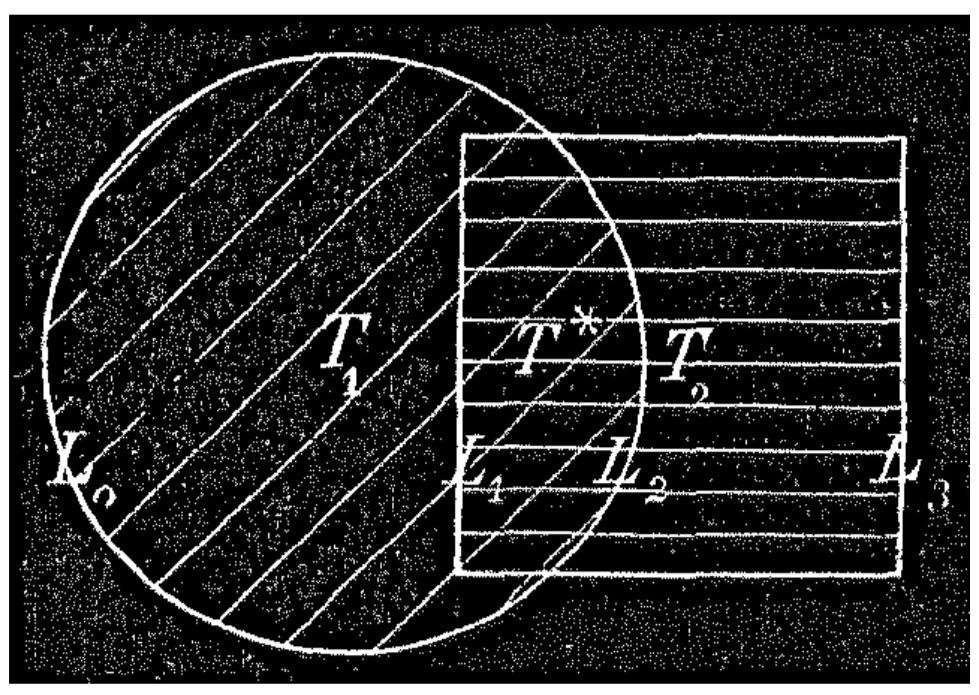
\includegraphics[scale=1.8]{original-drawing.png}
	\caption*{Original drawing by Schwarz} %(source: \cite{gander})}
\end{figure}
\end{frame}

\begin{frame}
\frametitle{Original Schwarz method}
\begin{columns}
\begin{column}{0.3\textwidth}
	\begin{figure}[h]
		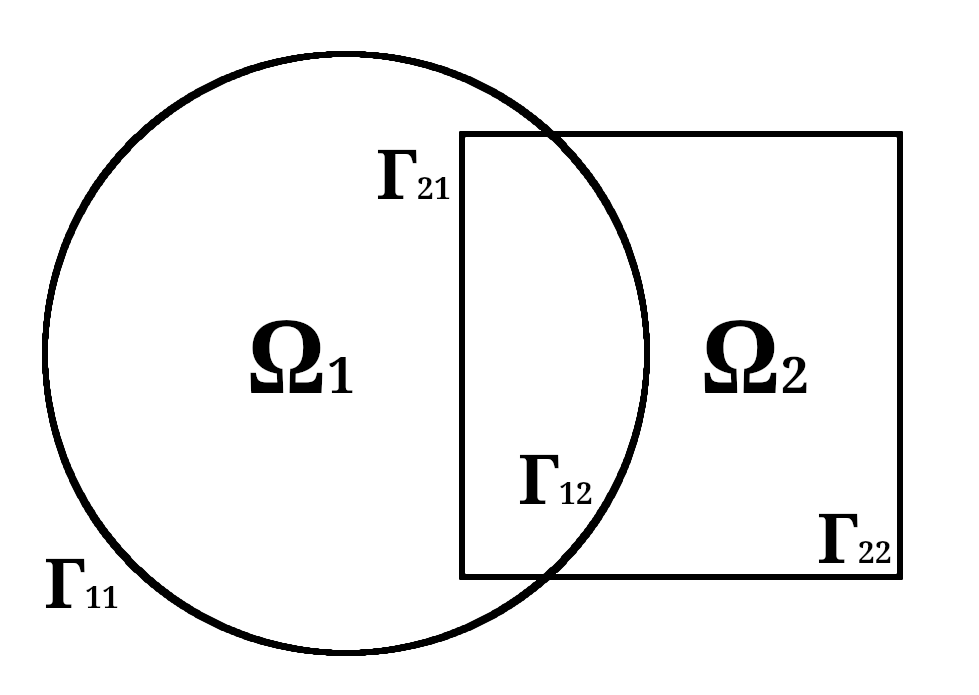
\includegraphics[scale=1.1]{modern-drawing.png}
		\caption*{The same drawing, with modern notation}
	\end{figure}
\end{column}
\begin{column}{0.5\textwidth}
\begin{align*}
&	u_1^0 = 0 \quad \text{in } \overline{\Omega_1} \\
&	u_2^0 = 0 \quad \text{in } \overline{\Omega_2} \\
&	\begin{cases}
		-\Delta u_1^n = f & \text{in $\Omega_1$} \\
		u_1^n = 0 & \text{on $\Gamma_{11}$} \\
		u_1^n = u_2^{n-1} & \text{on $\Gamma_{12}$}
	\end{cases} \\
&	\begin{cases}
		-\Delta u_2^n = f & \text{in $\Omega_2$} \\
		u_2^n = 0 & \text{on $\Gamma_{22}$} \\
		u_2^n = u_1^n & \text{on $\Gamma_{21}$}
	\end{cases}
\end{align*}
\end{column}
\end{columns}
\end{frame}

\begin{frame}
\frametitle{Original Schwarz method}
Let $u$ be the solution to Poisson's problem
\[
\begin{cases}
	-\Delta u = f & \text{in $\Omega = \Omega_1 \cup \Omega_2$} \\
	u = 0 & \text{on $\partial \Omega = \Gamma_{11} \cup \Gamma_{22}$} \\
\end{cases}
\]
Schwarz proved that $u_1^n \to u_{|\Omega_1}$ and $u_2^n \to u_{|\Omega_2}$
in $L^\infty$ at a geometric rate.
\pause

On the blackboard: if $u_1^n \to u_1$ and $u_2^n \to u_2$, then $u_1 = u_2$
on the overlap $\Omega_1 \cap \Omega_2$.
\pause

FreeFEM demo available in the file \texttt{original-schwarz.edp}
\end{frame}

\begin{frame}
\frametitle{Original Schwarz method}
List of 5 problems that we have to overcome:
\begin{enumerate}%[<+->]
\item[(1)] The algorithm is not parallel (as $u_2^n$ depends on $u_1^n$)
\item[(2)] The unknowns on the overlaps are duplicated
\item[(3)] The rate of convergence depends on the size of the overlaps
\item[(4)] We're not using state-of-the-art iterative sparse linear solvers
\item[(5)] The algorithm is not scalable as $N \to \infty$.
\end{enumerate}
% why poisson only?
% we will only cover poisson's eq.
% 1 hour is enough to explain the theory in full detail
% state of the art algorithm
% ideas can be applied to other PDEs (esp. elliptic)
% overlapping methods
\end{frame}

\begin{frame}
\frametitle{Original Schwarz method}
On the blackboard: two examples taken from Chapter 1.5 of \cite{nataf},
for which we compute the exact rates of convergence and show their
strong dependence on the size of the overlaps.

In the second example we also see how low-frequency modes of the error
converge to zero at a much slower rate than the high-frequency ones,
foreshadowing the need for a two-level method (as we will see shortly).
\end{frame}

\section{Jacobi-Schwarz, RAS, ASM}

\begin{frame}
\frametitle{Jacobi-Schwarz method}
If problem (1) is that $u_2^n$ depends on $u_1^n$, then we can fix it by
simply making it depend on $u_1^{n-1}$ instead:
\[
u_1^0 = 0 \quad \text{in } \overline{\Omega_1}
\qquad
u_2^0 = 0 \quad \text{in } \overline{\Omega_2}
\]
\[
\begin{cases}
	-\Delta u_1^n = f & \text{in $\Omega_1$} \\
	u_1^n = 0 & \text{on $\Gamma_{11}$} \\
	u_1^n = u_2^{n-1} & \text{on $\Gamma_{12}$}
\end{cases}
\qquad
\begin{cases}
	-\Delta u_2^n = f & \text{in $\Omega_2$} \\
	u_2^n = 0 & \text{on $\Gamma_{22}$} \\
	u_2^n = u_1^{n-1} & \text{on $\Gamma_{21}$}
\end{cases}
\]

We can again prove $L^\infty$ convergence at a (usually larger) \\ geometric rate.

FreeFEM demo available in the file \texttt{jacobi-schwarz.edp}
\end{frame}

\begin{frame}
\frametitle{Jacobi-Schwarz method}
Now we switch from the ``decompose, then discretize'' approach
to ``discretize, then decompose''. What happens at the linear algebra level?
Consider the system $Au = f$ associated with a
three-point finite differences scheme in 1D with step size $h$,
and consider the following domain decomposition with minimal overlap:
\[
\Omega = (0,1), \quad \Omega_1 = (0,(l+1)h),
\quad \Omega_2 = (lh,1), \quad l \in \mathbb{N} \cap [0,h^{-1}).
\]
We then partition all vectors and matrices accordingly (the first block
has size $l+1$, the other $h^{-1}-l$):
\[
A = \begin{pmatrix} A_{11} & A_{12} \\ A_{21} & A_{22} \end{pmatrix}
\quad
D = \begin{pmatrix} A_{11} & 0 \\ 0 & A_{22} \end{pmatrix}
\quad
u^n = \begin{pmatrix} u_1^n \\ u_2^n \end{pmatrix}
\quad
f = \begin{pmatrix} f_1 \\ f_2 \end{pmatrix}
\]
\end{frame}

\begin{frame}
\frametitle{Jacobi-Schwarz method}
Each Jacobi-Schwarz iteration corresponds to
\begin{gather*}
\begin{cases}
A_{11} u_1^n = f_1 - A_{12} u_2^{n-1} \\
A_{22} u_2^n = f_2 - A_{21} u_1^{n-1}
\end{cases} \\[6pt]
\begin{pmatrix} A_{11} & 0 \\ 0 & A_{22} \end{pmatrix}
\begin{pmatrix} u_1^n \\ u_2^n \end{pmatrix}
= \begin{pmatrix} A_{11} & 0 \\ 0 & A_{22} \end{pmatrix}
  \begin{pmatrix} u_1^{n-1} \\ u_2^{n-1} \end{pmatrix}
+ \begin{pmatrix} f_1 \\ f_2 \end{pmatrix}
- \begin{pmatrix} A_{11} & A_{12} \\ A_{21} & A_{22} \end{pmatrix}
  \begin{pmatrix} u_1^{n-1} \\ u_2^{n-1} \end{pmatrix} \\[6pt]
D u^n = D u^{n-1} + f - A u^{n-1} =\vcentcolon D u^{n-1} + r^{n-1} \\[6pt]
u^n = u^{n-1} + D^{-1} r^{n-1}
\end{gather*}
In numerical linear algebra, this iteration is known as the
block Jacobi algorithm. Hence the name Jacobi-Schwarz.
\end{frame}

\begin{frame}
\frametitle{Jacobi-Schwarz method}
In order to proceed further, we need to introduce additional notation.
%Let's find a way to express $D^{-1}$ in terms of $A$.

Let $n = \dim(A), \; m_i = \dim(A_{ii})$.

Let $R_i \colon \R^n \to \R^{m_i} \subset \R^n$ be the projections (or restrictions)
to the subspace associated with the degrees of freedom inside $\Omega_i$.

Then $R_i^{-1} = R_i^T$ and $A_{ii} = R_i A R_i^T$, so
\[
D^{-1}
= \sum_{i=1}^N R_i^T A_{ii}^{-1} R_i
= \sum_{i=1}^N R_i^T (R_i A R_i^T)^{-1} R_i
\]

However, this is no longer true if the overlap is not minimal,
as the blocks $A_{ii}$ will not be disjoint anymore.
We double-count (or worse) on the overlaps $\Omega_i \cap \Omega_j$.
\end{frame}

\begin{frame}
\frametitle{Jacobi-Schwarz method}
We can solve this problem by introducing a \emph{discrete partition of unity}:
a set of matrices $D_i \colon \R^{m_i} \to \R^{m_i}$ such that
\begin{align*}
&	D_i \geq 0 \quad \forall i = 1,\dots,N \\
&	I = \sum_{i=1}^N R_i^T D_i R_i
\end{align*}
Now
\[
D^{-1}
= \sum_{i=1}^N R_i^T D_i A_{ii}^{-1} R_i
= \sum_{i=1}^N R_i^T D_i (R_i A R_i^T)^{-1} R_i
\]
is always true, even if the blocks $A_{ii}$ overlap.

\end{frame}

%\begin{frame}
%\frametitle{Restricted Additive Schwarz method (RAS)}
%RAS is an algorithm equivalent to Jacobi-Schwarz
%\begin{align*}
%&	u^0 = 0 \quad \text{in } \overline{\Omega}
%	\qquad u^n = \sum_{i=1}^N E_i(\chi_i w_i^n) \\
%&	\begin{cases}
%		-\Delta w_i^n = f & \text{in $\Omega_i$} \\
%		w_i^n = 0 & \text{on } \partial\Omega_i \cap \partial\Omega \\
%		w_i^n = u^{n-1} & \text{on the rest of the boundary}
%	\end{cases}
%\end{align*}
%
%Live FreeFEM demo
%\end{frame}

\begin{frame}
\frametitle{Additive Schwarz Method (ASM)
	and Restricted Additive Schwarz (RAS) preconditioners}
The iterative method $u^n = u^{n-1} + D^{-1} r^{n-1}$
is known as \emph{overlapping block Jacobi}.
Since Krylov-space methods (e.g.\ CG) always converge faster than
fixed point iterations (like block Jacobi),
we define the two following preconditioners:
\[
M_\text{RAS}^{-1} = \sum_{i=1}^N R_i^T D_i (R_i A R_i^T)^{-1} R_i
\]
\[
M_\text{ASM}^{-1} = \sum_{i=1}^N R_i^T (R_i A R_i^T)^{-1} R_i
\]
Note that block Jacobi is equivalent to Richardson's method
with one of these preconditioners.
\end{frame}

\begin{frame}
\frametitle{Additive Schwarz Method (ASM)
	and Restricted Additive Schwarz (RAS) preconditioners}
$M_\text{ASM}^{-1}$ is not as good as $M_\text{RAS}^{-1}$, but it's
still useful in practice because it's symmetrical
(and so it can be used with the conjugate gradients method,
just to give an example).

The preconditioning approach greatly reduces the coupling
between the convergence ratio and the size of the overlaps
(see Figure 3.1 in \cite{nataf}),
so we can consider problems (2), (3) and (4) solved by now.

Regarding the eigenvalues of the preconditioned system,
we can bound $\lambda_\text{max}$ from above with a constant
that doesn't depend on $N$ (as in Lemma 5.9 of \cite{nataf}),
but it's still not possible to bound $\lambda_\text{min}$ from below
without additional hypothesis. Hence problem (5) is still open.
\end{frame}

\section{Two-level methods to the rescue}
\begin{frame}
\frametitle{The need for a two-level method}
The preconditioner $M_\text{ASM}^{-1}$ is still not scalable.
When applied to Richardson's scheme, it's easy to see that information
from one subdomain flows only to its direct neighbors.
As the number of subdomains grows, so does the minimum number of iterations required
to get a global exchange of information.
The preconditioned matrix $M^{-1}A$ has a few small eigenvalues that cause
the norm of the residual to plateau when using an iterative scheme.
Solution: couple all subdomains by introducing a new, non-localized
term to $M$ (a so-called \emph{coarse-space correction}).
\end{frame}

\begin{frame}
\frametitle{Nicolaides coarse space}
In the case of Poisson's equation, the small eigenvalues
of $M^{-1}A$ come from piecewise constant functions
(i.e.\ the kernel of the Laplace operator on the subdomains).

How can we use this information to get a better $M$?
\end{frame}

\begin{frame}
\frametitle{Nicolaides coarse space}
Let $Z$ be the matrix whose columns form a basis for the vector space
of piecewise constants functions on the $N$ subdomains
(the \emph{Nicolaides coarse space}):
\[
Z_i = R_i^T D_i R_i \;\! \textbf{1}
\]
Let $y$ be an approximate solution to the linear system $Au = f$,\\
and let $r$ be the residual $f-Ay$. Consider the problem of finding
the best correction for $y$ (in the energy norm)
among the space of piecewise constants functions:
\[
\min_{\beta \in \R^N} \norm{y+Z\beta-u}_A
\]
\end{frame}

\begin{frame}
\frametitle{Nicolaides coarse space}
Since $A$ is SPD (discretization of $-\Delta$), the minimum is given by
\[
\beta = (Z^TAZ)^{-1} Z^T r,
\]
and the best correction for $y$ is
\[
Z\beta = Z (Z^TAZ)^{-1} Z^T r.
\]
Notice how similar this looks to the expression for $M_\text{ASM}^{-1}$!
\end{frame}

\begin{frame}
\frametitle{Two-level additive Schwarz preconditioner}
This observation suggests the following definition of a two-level
additive Schwarz preconditioner:
\[
M_\text{ASM,2}^{-1} = Z (Z^TAZ)^{-1} Z^T + \sum_{i=1}^N R_i^T (R_i A R_i^T)^{-1} R_i
\]
It's now possible to prove that $M_\text{ASM,2}^{-1}$ is a scalable preconditioner
(see e.g.\ Corollary 5.12 in \cite{nataf}).

FreeFEM demo available in the file \texttt{AS2-PCG.edp}
\end{frame}

\begin{frame}
\frametitle{Two-level additive Schwarz preconditioner}
Has problem (5) been solved? \\
Did we finally get an algorithm that scales, as $n \to \infty$?
\pause

Almost. The devil is in the details...
\pause

We need to factorize $Z^TAZ$, an $N \times N$ matrix.
As $n \to \infty$ implies $N \to \infty$, this a very difficult problem
to solve in a scalable way (because it's just as hard as factorizing $A$
in the first place).
\pause

Three-level methods to the rescue?
\pause

Not necessarily, unless $N$ is greater than the number of degrees of freeedom
assigned to each subdomain $\Omega_i$.
How large is the problem that we want to solve, anyway?
\end{frame}

\section{Beyond Poisson's equation}
\begin{frame}
\frametitle{Beyond Poisson's equation}
Here are some advanced concepts that we didn't cover during this presentation,
but nevertheless deserve to be mentioned:
\begin{itemize}
\item Optimized Schwarz methods (subdomains share information through
	Robin boundary conditions instead of Dirichlet)
\item Spectral coarse spaces (a generalization of Nicolaides spaces, defined
	by harmonic extensions of the eigenvectors corresponding
	to small eigenvalues of the Dirichlet-to-Neumann map in each subdomain)
\item Neumann–Neumann and FETI algorithms (they require
	nonoverlapping domain decompositions)
\item The GenEO method (can build robust and efficient coarse spaces
	by solving generalized eigenvalue problems)
\end{itemize}
\end{frame}

\begin{frame}
\frametitle{Beyond Poisson's equation}
Besides Poisson's equation, domain decomposition methods have been
successfully applied to:
\begin{itemize}%[<+->]
\item Helmholtz equation
\item Biharmonic equation
\item Equilibrium equations of linear elasticity
\item Stokes equations
\item Maxwell's equations in time-harmonic form
\end{itemize}
and more. Understanding how DDM can be best applied to different kinds of
PDEs is currently the subject of ongoing research.
\end{frame}

\begin{frame}
\frametitle{Domain decomposition, in practice}
HPDDM is a C++ library that implements various domain decomposition methods,
with a focus on performance. It's well integrated with PETSc, Trilinos and FreeFEM
(using the \texttt{ffddm} plugin).
The first version of the software was written by Pierre Jolivet and Frédéric Nataf,
two of the authors of \cite{nataf}.
\end{frame}

\begin{frame}
\frametitle{Bibliography}
\begin{thebibliography}{9}
\bibitem{nataf} Dolean, V., Jolivet, P., \& Nataf, F.\ (2015).
An introduction to domain decomposition methods: algorithms,
theory, and parallel implementation (Vol.\ 144). SIAM.
\bibitem{gander} Gander, M.\ J., \& Wanner, G.\ (2014).
The origins of the alternating Schwarz method.
\bibitem{widlund} Widlund, O., \& Dryja, M.\ (1987).
An additive variant of the Schwarz alternating method for the case of many subregions.
\bibitem{nicolaides} Nicolaides, R.\ A.\ (1987).
Deflation of conjugate gradients with applications to boundary value problems.
\bibitem{lions} Lions, P.\ L.\ (1989).
On the Schwarz alternating method II.
\end{thebibliography}
\end{frame}

\begin{frame}
\frametitle{That's all folks}
\begin{center}
Thank you for your attention! \\[14pt]
Are there any questions?
\end{center}
\end{frame}











%\begin{frame}
%\frametitle{Grafo delle implicazioni}
%\begin{equation*}
%\begin{tikzcd}[ampersand replacement=\&, row sep = large, column sep = large]
%\text{Soluzioni $L^p$} \ar[rd, "1"]
%	\& \text{$\norm{S(t)}$ in $L^p$} \ar[l] \\
%\text{Esp. Stab.} \ar[u] \ar[d]
%	\& \text{Unif. Esp. Stab.} \ar[u] \ar[d, shift left] \ar[l] \ar[r,shift right]
%	\& \text{Unif. Stab.} \ar[l,shift right,swap,"2"] \\
%\text{Stab.}
%	\& s(A)<0 \ar[u, shift left, dashed, "3"]
%\end{tikzcd}
%\end{equation*}
%\begin{enumerate}
%\item<2-> Teorema di Datko (1970).
%\item<3-> Esiste $t_0 \geq 0$ tale che $\norm{S(t_0)} < 1$.
%\item<4-> È sufficiente mostrare che $\omega_0(A) = s(A)$.
%\end{enumerate}
%\end{frame}

\end{document}




























